\section{Our Current Data Disguising Framework}

We propose \emph{data disguising}, a systematic approach to privacy transformations
that separates them from application code.
%
We believe that data disguising systems will help support flexible privacy
transformations.
%
Data disguising represents privacy transformations as structured \emph{disguises}
that the application developer specifies to capture an application's privacy policies.
%
Applications invoke an external data disguising tool's API to apply disguises; the tool
interprets the specification and applies the necessary physical changes to the
database.
%
Data disguising offers mechanisms to handle interactions between disguises and
reversible disguises.
%in the form of automatically-generated \emph{revealing functions} stored in \emph{vaults}.

%
%In the following, we sketch one design for a data disguising framework.
%
%Some of the specific design decisions in this framework have alternatives that are worth
%investigating, and open research questions remain; we discuss these in \S\ref{s:disc}.

\subsection{Disguises: Structured Privacy Transformations}
\label{sec:disguises}

\begin{figure}[t]
    \centering
    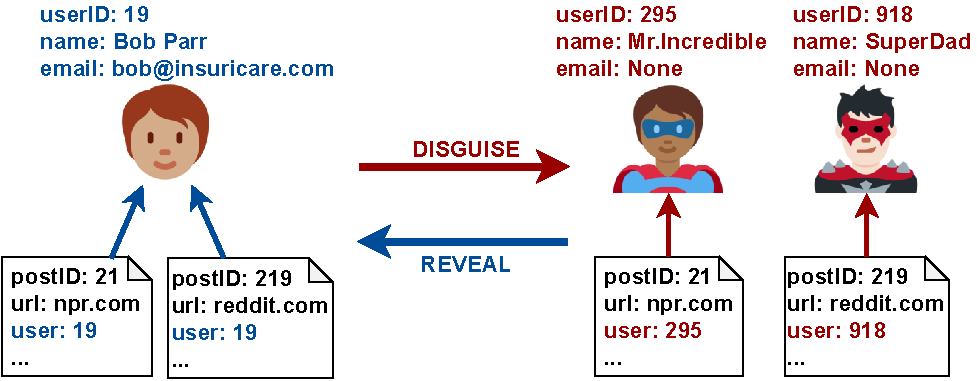
\includegraphics[width=0.47\textwidth]{img/disguises_new}

    \caption{HotCRP's user scrubbing disguise decorrelates Bea's reviews from Bea's identity while maintaining
    referential integrity using anonymous placeholders.}
    \label{fig:example}
\end{figure}

\begin{figure}[t!]
    \centering
    \footnotesize
\begin{lstlisting}[language=Rust]
disguise_name: "UserScrub",
user_to_disguise: $UID,
tables:
   ContactInfo:
      generate_placeholder: [
         ("name", Random),
         ("email", Default(None)),
         ("active", Default(false)),
         ..
      ],
      transformations: [Remove(pred: "contactId" = $UID)]
   ReviewPreference:
      transformations: [Remove(pred: "contactId" = $UID)]
   Review:
      transformations: [Decorrelate(
         pred: "contactId" = $UID,
         foreign_key: ("contactId", ContactInfo)
      )]
\end{lstlisting}
    \caption{Part of a HotCRP user scrubbing disguise specification. \texttt{\$UID} refers
    to the user invoking the disguise.}
    \label{fig:spec}
\end{figure}

%
The broad range and application-specific nature of privacy transformations poses a real
implementation challenge.
%
Most importantly, transformations must maintain the integrity of the application's data
in storage when applied.
%
For example, decorrelating users from their reviews could easily violate referential
integrity (\ie no dangling foreign keys) unless applied carefully.
%
%We believe that data disguising makes privacy transformations more manageable by
%separating them from application code, and
%
Data disguises' structured nature, and automated application, seeks to ensure this
property.
%

%
Data disguises are built on three fundamental operations---data removal, object content
modification, and decorrelation by modifying references between objects---that can
capture and structure many desirable privacy transformations.
%
The application developer writes a disguise specification for each of the application's
privacy transformations.
%
This specification consists of predicated operations on each table, and describes
the necessary operations to perform on objects that satisfy the predicate.
%
The data disguising tool takes the disguise specification and turns it into storage
operations that appropriately rewrite affected foreign keys.
%

%
Figure~\ref{fig:example} illustrates how the tool performs the example user
account deletion disguise for Bea, when given a specification like that in Figure~\ref{fig:spec}.
%
When her account is active, Bea's profile is associated with her true identity and her
reviews.
%
When Bea deletes her account, her reviews move to privacy-preserving
placeholders, making it seem as if a different user entered each of Bea's reviews.
%
This prevents an observer from correlating these contributions to expose Bea's identity,
but importantly preserves referential integrity.
%

%
%Disguises transform a guise by modifying it at per-attribute (\ie per-column) granularity, or
%splitting it into multiple guises in order to decorrelating from objects that reference it (via \eg foreign-key relationships).
%
%Guises can also be removed entirely.
%
%At any given moment, an application's data comprises a mix of identity-revealing guises
%and privacy-preserving ones. Disguises modify, split, and/or combine individual guises when triggered.

%-------------------------------------------------------------------------------
\subsection{Handling Disguise Interactions}
%\label{sec:composition}
%-------------------------------------------------------------------------------

Applications use disguises to achieve specific privacy goals, but this can be
complicated by interactions between different disguises.
%
Because disguises inherently reduce identifying information,
applying one disguise may change the outcome of future disguises applied on top of it.
%

%
For example, consider two desirable disguises in HotCRP: \gdpr and \ca.
%
\gdpr removes a user's account (\S\ref{design:eg}); \ca provides user privacy by
anonymizing all conference data.
%
These disguises touch the same data: applying \ca destroys information that \gdpr would
remove or transform if applied to an unmodified database.
%

%
In some cases, the disguises compose naturally---\eg there is no need to decorrelate
data that another disguise removed---but in others, the tool may need to access the
original data to meet the application's privacy goals.
%
%Even then, the necessary actions depend on the specific application:
%some applications may require that previously anonymized data still be deleted, while other
%applications may not.
%
Data disguising provides the infrastructure and mechanisms to reveal data in support
of disguise composition; however, detecting automatically when this is needed to
achieve application privacy goals remains an open challenge (\S\ref{s:disc}).
%To handle inter-disguise dependencies, a disguising tool relies on (1) the structured nature of
%disguises to
%statically determine whether disguises share dependencies, and (2) the key abstraction of \emph{user
%vaults}, namely per-user logs of disguise updates to that user's data.  User vaults solve the issue
%that disguises inherently destroy data necessary to correctly achieve the end-state of future
%disguises by providing a secure way to store the data. A disguising tool queries the user vault to
%temporarily restore destroyed data (\eg decorrelated foreign key relationships) in order to apply
%the disguise correctly.

%As shown in Figure~\ref{fig:tool}, a disguising tool sits next to the application, and queries the
%user vaults and the application database. The application performs disguises by invoking a
%disguising tool.

%-------------------------------------------------------------------------------
%\paragraph{Vaults.}
%-------------------------------------------------------------------------------
%
\textbf{Vaults} provide the infrastructure to reveal previously disguised data
when necessary.
%, either for temporary data for disguise composition, or for reversing a disguise entirely.
%
A vault is a storage location not accessible to application queries that stores
\emph{reveal functions} for applied disguises.
%
Applying these functions reveals the underlying data transformed by a disguise
(possibly temporarily).
%
%These functions are automatically produced by the disguising tool when a disguise is applied.
The disguising tool generates the reveal functions when applying a disguise, using
the specification and the disguised data.
%

%
Vaults admit various deployment models that have different security and privacy
properties.
%
%It remains important, however, that any configuration of vaults should not violate the
%guarantee that disguises indeed destroy data, from the viewpoint of the application and
%any users.
%
These include storing vaults in offline storage, which provides a modicum of security,
but makes access by the data disguising tool easy; or having vaults stored entirely by
some third party or locally by the user, with an API for disguise tool access.
%
Further, the vault contents might be encrypted, and access might require explicit approval
by the user, who holds the private key.
%
To protect against lost keys, the private key could be secret-shared~\cite{secretsharing}
between the user, the web application, and a trusted third party (\eg the EFF), so that
the user can authorize the applicaiton and the third party to restore the key.
%
Entries in a vault could also be configured to expire after some time; making the
corresponding disguises irreversible.
%

%
The vault deployment model has serious consequences for the practicality of disguise
reversal.
%
For example, a reversible \gdpr requires reveal functions stored in per-user vaults
external to the application storage in order to be GDPR-compliant.
%
While it is reasonable to imagine accessing a single user's vault to reverse \gdpr in
this model, complete reversal of \ca would need to retrieve revealing functions from
all users' vaults, an infeasible task.
%
An alternative might be a multi-tier security design: the first tier stores revealing
functions of non-GDPR disguises in a global vault accessible to the disguising tool
and application, while the second tier stores revealing functions from user-invoked
disguises in external, per-user encrypted vaults.
%
We imagine that exploring different vaults designs will be an important part of
data disguising research.
%

%-------------------------------------------------------------------------------
%\paragraph{Revealing Data.}
%-------------------------------------------------------------------------------
%\lyt{I feel like this sticks out, but it is a reasonable part of our solution to handling disguise
%reversal.}
\textbf{Reverting disguises.}
%
Reveal functions also help with explicit disguise reversal (\eg a returning user): the
application invokes the disguising tool's API to revert a previously applied disguise.
%
This reversal permanently reveals data, restoring it to the application database.
%
However, other disguises may have affected the database contents in the interval between
the original disguising and the explicit reveal.
%
To ensure that any revealed data still respects other active disguises, the tool keeps
a persistent log of all disguises the application applied, and re-applies disguises from
the relevant log interval to the revealed data.
%

%
For example, reversal of \gdpr must avoid reintroducing identifiable reviews if \ca has
occurred since \gdpr was applied.
%
The data disguising tool would applying the relevant \ca anonymization operations to any
revealed data from \gdpr's reversal before making it visible the application.
%

%
Explicit application modifications to disguised data (other than deletion) are harder to
handle; the framework might prohibit them, or log them to the relevant vaults.
%

%\ms{OLD TEXT FOLLOWS}

\iffalse
%For example, Figure~\ref{fig:example} would include a specification that all email
%addresses be obfuscated in an anonymous manner for the user with name ``Bob Parr''.
%
%Transformations can either remove objects, or change objects into one or more guises.
%To create a guise from an object, developers specify how to transform attributes of the
%object (\eg table column values) into guise attributes (\eg changing email addresses).

%
%When writing a disguise, developers can reason about its
%specification in isolation; interactions between different disguises are handled by a disguising
%tool (\S\ref{sec:composition}).
%
%We assume that:
%\begin{enumerate}[nosep]
%  \item developers use their domain knowledge to write correct and complete disguises;
%      \lyt{should make clear that correct/complete is just operational? \eg doesn't mess up the DB}
%  \item application code handles the different guises appropriately (\eg in
%    displaying them); and
%  \item different guises of the same object have the same structure (\eg they can be
%    rows in the same table).
%\end{enumerate}
%
Developers choose how to create other guise attributes, selecting from among the following:
%
\paragraph{(1) Copy object content.}
%
Guises of the same object all share the object's attribute values.
%
If the attribute is a reference attribute (\eg a foreign key column), all guises will refer to the same object.
%
%
Copying allows developers to retain the object's content, without worrying about how to
synthesize attribute values for guises.
%
%However, this should only be chosen if guise attribute
%values cannot be generated, or if this attribute says little about the true identity of the
%entity.
For example, in Figure~\ref{fig:guises} the \texttt{darkmode} attribute is copied in
all guises.
%; the \texttt{darkmode} attribute reveals very little about the underlying user's
%identity.

\paragraph{(2) Generate new content.}
%
To create new attributes, developers specify whether the guise's value should be random,
a default value, or generated from the object's attribute value via a custom function (\eg hashing
the value).
%
Figure~\ref{fig:guises} illustrates an example of random (\texttt{name}) and default
(\texttt{active}) generated value attributes.
%
%
Creating new guise reference attributes (\eg new foreign key relationships) requires
creating a new guise for the referenced object in order to maintain referential
integrity;
the data disguise rewrites the reference to point to the new guise.
%
In Figure~\ref{fig:guises}, creating two user guises requires creating two
tag guises, and the tag guises' identifiers become the user guises' foreign keys.
%

\paragraph{(3) Copy object content, but only once.}
%
One guise copies the attribute value from the object, but all other guises generate new
values (as described above).
%
\texttt{notifs} in Figure~\ref{fig:guises} illustrates how the attribute is copied once.
%
This enables the application to retain the original object semantics (\eg a count of how many
users want notifications) without creating duplicates.
%



\begin{figure*}[t!]
    \centering
    \footnotesize
\begin{tabular}{@{}c|c|c|c@{}}
\textbf{User Transformation Spec} & \textbf{User Object} & \textbf{Guise 1} &
    \textbf{Guise 2} \\
\begin{lstlisting}[language=Rust]
"id":       IDAttribute,
"name":     Gen(Random),
"active":   Gen(Default(false)),
"darkmode": CopyAll,
"notifs":   CopyOnce+Gen(Default(false)),
"tag_id":   GenForeignKey,
\end{lstlisting}
    &
\begin{lstlisting}[language=Rust]
"id":       19,
"name":     BobParr,
"active":   true,
"darkmode": false,
"notifs":   true,
"tag_id":   11
\end{lstlisting}
&
\begin{lstlisting}[language=Rust]
"id":       295,
"name":     MrIncredible,
"active":   false,
"darkmode": false,
"notifs":   true,
"tag_id":   81483
\end{lstlisting}
&
\begin{lstlisting}[language=Rust]
"id":       918,
"name":     SuperDad,
"active":   false,
"darkmode": false,
"notifs":   false,
"tag_id":   15592
\end{lstlisting}
\end{tabular}
    \caption{Creating two guises of an example user (of a synthetic application schema).}
    \label{fig:guises}
\end{figure*}


%-------------------------------------------------------------------------------
\paragraph{Applying Disguises.}
%-------------------------------------------------------------------------------
A disguising tool applies disguises in a five-phase procedure:
\begin{enumerate}[nosep]
    \item \emph{Prepare}: execute the appropriate reveal functions of co-dependent,
        reversible disguises from the user vaults, if applicable (\S\ref{sec:composition})
        %reconcile any data dependencies between this disguise and prior disguises.
        %A disguising tool detects read-after-write dependencies between the new disguise's
        %predicates and prior disguises' updates, and, using entries in the vault, undoes any writes
        %that may affect the new disguise's predicates. As an optimization, vault entries recording
        %object removals need not be reversed.
        \item \emph{Read}: get all objects that satisfy (per-type) developer-specified predicates.
        \item \emph{Update}: modify, decorrelate, or remove objects read in step (2) according to the
        developer's specification.
    \item \emph{Record}: if the disguise is reversible, store per-user reveal functions for the
        disguise in the appropriate per-user vaults.
        A disguising tool must be able to determine which user vault should record each modification. This can be
        developer-specified, or rely on a set of heuristics (\eg assigning ownership by traversing,
        starting from each user, the application's object graph expressed in an object-relational
        model (ORM)~\cite{orm}, or implicitly via foreign keys).
        \item \emph{Finalize}: After applying the new disguise updates, the disguising tool
            redisguises any temporarily revealed data from earlier disguises.
\end{enumerate}

%Composed disguises should achieve an end-state that combines, in some way, the end-states achieved by each disguise when applied to the original application database in isolation.
%Correct composition of multiple disguises achieves an end-state equivalent to combining the
%end-states achieved by each disguise when applied to the original application database in isolation.
%
%If a prior disguise is reversible, then a disguising tool can use user vaults to ensure that this
%prior disguise does not affect \emph{which} objects are updated
%a future disguises.
%%In this case, a disguising tool allows developers to reason about multiple conflicting updates to
%the same object:
%regardless of when the disguises occurred, if one disguise removes an object that the other disguise
%modified, then the removal takes precedence.
%%
%
%However, if they both modify the same object attribute, a disguising tool establishes no precedence
%between the modifications and applies them in chronological order.  Alternatively, we can imagine
%that the developer could specify a partial ordering between modifications, or our framework could
%restrict the set of possible modifications and establish a precedence order within this set.
%
%If the prior disguise is not reversible, however, then the disguising tool could prevent future
%conflicting disguise application, or perhaps a-priori prevent the application of such non-reversible
%disguises that conflict with legally required disguises such as GDPR deletion \lyt{not sure what to
%put here? May also want to include something about developer assertions}
%%: a disguise will update all objects that it would have updated if performed on
%the original, undisguised state of application data.


\fi
